\subsection{Away-step comparison from the original point}
The initialization study motivates a direction-level control. We compare
FW and AFW, each with ordinary backtracking (BT) or the explicit
known-$H$ quadratic step (Q), on the same 70 instances. All four methods
start at the original vertex, without a compulsory initial move.
BT starts at estimate 1, halves before each search, and doubles on
rejection. Q uses $H_0+H_1U_k$. AFW chooses the stronger FW/away
direction and respects its active-weight cap. The certificate uses the
full FW gap even on away steps. This is an implementation of established
algorithms, not a newly proposed AFW direction rule.

The 280 runs include 140 exact repeats of the earlier two FW baselines,
verified against their saved objectives, certificates and oracle counts.
The 140 AFW runs add method comparisons on existing instances, rather
than new independent tasks. Table~\ref{tab:away} distinguishes the
outer cap of 1000 updates from a fixed budget of 1000 function calls.
The budget values use complete trajectory prefixes. Function, gradient
and full-LMO calls are reported separately; each method uses $N+1$
gradients and full LMOs. AFW additionally scans its active set once per
update, and records the number of atom scores. Maintaining and
reconstructing active weights also costs work, so oracle counts alone
do not establish a wall-clock advantage.

AFW-BT reaches $U\le10^{-5}$ in all 70 runs within the outer cap.
On the scaled active family, it certifies 10/10 instances, using medians
56.5 function calls and 28.5 gradients. FW-BT certifies none within the
cap. On the breast-cancer control, AFW-BT certifies 10/10 with 103.5
median function calls, versus 0/10 for FW-BT. On Bike Sharing AFW-BT
certifies 10/10 by the end, but only 6/10 at 1000 function calls; the
corresponding FW-BT count at that budget is 1/10. End-of-run medians
include capped runs and must be read with these successes.

AFW-Q still certifies no run of either real regression within 1000
updates. Thus active-set correction alone does not make a conservative
analytic step efficient on these data. On the interior family, the
FW/AFW differences are modest. Figure~\ref{fig:away} shows the fixed
function-budget profiles; it does not establish a ranking over all
projection-free methods or untested instances.

Every step of the 70 AFW-BT trajectories is checked before trace
sampling: accepted-curvature envelope, dyadic trial identity, local
decrease, phase lag budget, drop count, and total function-call bound.
The certificate bridge is checked using the independent reference
interval and the analytically valid ridge lower bound on strong
convexity. No positive weights are pruned heuristically in these runs,
and no unexpected numerical atom deletions occur. A separate interval
test, where the geometric width is explicit, checks
\eqref{eq:awaygeometry} and the strongly convex phase bound. A geometric
constant is not fitted to the benchmark trajectories, and these finite
checks do not independently validate the general theorem.

\begin{table}[htbp]
\centering\small
\caption{FW versus AFW from the same original point, ten matched seeds. Final medians include capped runs; the cap is 1000 updates. The last columns use a separate budget of 1000 function calls.}
\label{tab:away}
\begin{tabular}{lrrrrr}
\hline
Method & Final successes & $f$ calls & $\nabla f$ calls & Successes at 1000 $f$ & Median $U$ \\
\hline
\multicolumn{6}{l}{\textbf{active\_scaled}} \\
FW\_BT & 0/10 & 2002.0 & 1001.0 & 0/10 & 3.28e-03 \\
AFW\_BT & 10/10 & 56.5 & 28.5 & 10/10 & 7.94e-06 \\
FW\_Q & 0/10 & 1001.0 & 1001.0 & 0/10 & 4.26e-03 \\
AFW\_Q & 10/10 & 160.5 & 160.5 & 10/10 & 8.67e-06 \\
\hline
\multicolumn{6}{l}{\textbf{breast\_cancer}} \\
FW\_BT & 0/10 & 1997.0 & 1001.0 & 0/10 & 3.11e-04 \\
AFW\_BT & 10/10 & 103.5 & 53.5 & 10/10 & 9.52e-06 \\
FW\_Q & 0/10 & 1001.0 & 1001.0 & 0/10 & 8.67e-03 \\
AFW\_Q & 0/10 & 1001.0 & 1001.0 & 0/10 & 1.24e-03 \\
\hline
\multicolumn{6}{l}{\textbf{bike\_poisson}} \\
FW\_BT & 8/10 & 1789.0 & 894.5 & 1/10 & 3.01e-05 \\
AFW\_BT & 10/10 & 877.5 & 439.0 & 6/10 & 9.88e-06 \\
FW\_Q & 0/10 & 1001.0 & 1001.0 & 0/10 & 1.04e-01 \\
AFW\_Q & 0/10 & 1001.0 & 1001.0 & 0/10 & 1.00e-01 \\
\hline
\end{tabular}
\end{table}

\begin{figure}[htbp]
\centering
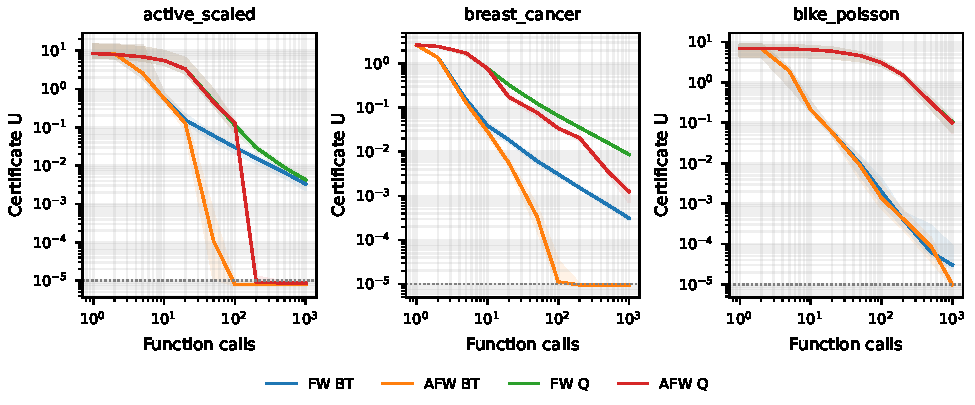
\includegraphics[width=\textwidth]{figures/away_comparison.pdf}
\caption{FW versus AFW from a common original start. Median certificate
and interquartile band at displayed function-call budgets. Completed
runs are carried forward. Every nonterminal run reaches the displayed
budgets before the outer cap. Lines between budgets are for display;
the CSV stores actual available certificates. Q methods receive analytic
curvature constants; BT methods do not. Active-set work is additional.}
\label{fig:away}
\end{figure}
